% Created 2021-01-13 mer. 22:12
% Intended LaTeX compiler: pdflatex
\documentclass[11pt]{article}
\usepackage[utf8]{inputenc}
\usepackage[T1]{fontenc}

\usepackage[a4paper,bindingoffset=0.5in,%
            left=0.5in,right=0.5in,top=1in,bottom=1in,%
            footskip=.25in]{geometry}

\usepackage{graphicx}
\usepackage{amsmath}
\usepackage{amssymb}
\usepackage{xspace}
\usepackage{commath}
\usepackage{times}
\usepackage{bm} 
\usepackage{balance}
\usepackage{hyperref}
\usepackage{mathtools}
\usepackage{stmaryrd}
\usepackage{wasysym}
\usepackage{soul}

\usepackage[toc,page]{appendix}

%%%% Define Acronyms
\usepackage{acronym}
%
\newacro{DF}{distribution fonction}

\newcommand{\bv}{\boldsymbol{v}}
\newcommand{\bnab}{\boldsymbol{\nabla}}
\newcommand{\rd}{\mathrm{d}}
\newcommand{\vr}{v_{r}}
\newcommand{\vt}{v_{\theta}}
\newcommand{\Sigmad}{\Sigma_{\rm{disk}}}
\newcommand{\Sigmadh}{\Sigma_{\rm{DH}}}
\newcommand{\Phib}{\Phi_{\rm{bulge}}}
\newcommand{\Phid}{\Phi_{\rm{disk}}}
\newcommand{\Phidh}{\Phi_{\rm{DH}}}
\newcommand{\Phisg}{\Phi_{\rm{sg}}}

\newcommand{\Mb}{M_{\rm{bulge}}}
\newcommand{\Md}{M_{\rm{disk}}}
\newcommand{\Mdh}{M_{\rm{DH}}}
\newcommand{\Msg}{M_{\rm{sg}}}

\newcommand{\anm}{a_n^m}
\newcommand{\bnm}{b_n^m}
\newcommand{\cnm}{c_n^m}
\newcommand{\alm}{a_l^m}
\newcommand{\blm}{b_l^m}
\newcommand{\clm}{c_l^m}
\newcommand{\Pnm}{P_n^{|m|}}
\newcommand{\Plm}{P_l^{|m|}}
\newcommand{\hPnm}{\widehat{\Pnm}}
\newcommand{\hPlm}{\widehat{\Plm}}
\newcommand{\hI}{\widehat{I}}
\newcommand{\hJ}{\widehat{J}}
\newcommand{\hIp}{\widehat{I'}}
\newcommand{\hJp}{\widehat{J'}}

\newcommand{\homega}{\widehat{\omega}}
\newcommand{\hOmega}{\widehat{\Omega}}
\newcommand{\Omegaref}{\Omega_{\mathrm{ref}}}
\newcommand{\hkappa}{\widehat{\kappa}}

\newcommand{\Sigmaref}{\Sigma_{\mathrm{ref}}}
\newcommand{\hSigma}{\widehat{\Sigma}}


\author{Kerwann}
\date{\today}
\title{Notes}
\hypersetup{
 pdfauthor={Kerwann},
 pdftitle={Notes},
 pdfkeywords={},
 pdfsubject={},
 pdfcreator={Emacs 27.1 (Org mode 9.3)}, 
 pdflang={English}}
\begin{document}

\maketitle

\tableofcontents


\section{Self-gravitating thin disk with constant stellar mass}
\label{sec:sg_disk_cst_mass}



\subsection{Case $\Gamma=4/3$}

Consider a self gravitating disk with surface density $\Sigma$ and gravitational potential $\Phi$. Let $\bv$ be its velocity field and $P$ its pression field. Then it is described by the system
\begin{align}
&\frac{\partial \Sigma}{\partial t} + \bnab \cdot (\Sigma \bv) = 0 ,\\
&\frac{\partial \bv}{\partial t} + (\bv \cdot \bnab)(\bv) = -\frac{1}{\Sigma} \bnab P - \bnab \Phi ,\\
& \Delta \Phid = 4\pi G \Sigma \delta (z).
\end{align}
Here, $\Phi =\Phib^0+  \Phid +  \Phidh^0$. 
Suppose that we have a polytrope gas such that $P=\alpha \Sigma^{\Gamma}=\alpha \Sigma^{4/3}$ and let
\begin{equation}
\psi = \int \frac{\rd P(\Sigma)}{\Sigma} \Leftrightarrow \bnab \psi = \frac{\bnab P}{\Sigma}.
\end{equation}
 Then
 \begin{equation}
\psi = 4\alpha \Sigma^{1/3}.
\end{equation}
 
 Letting $\Psi = \Phi + \psi$, we obtain
\begin{equation}
\frac{\partial \bv}{\partial t} + (\bv \cdot \bnab)(\bv) = - \bnab \Psi.
\end{equation}

%If $\Sigma_{\rm{disk}}\propto\Sigma_{\rm{DH}}$ then $q\in [1,+\infty[$ is constant and $q=1+\Mdh/\Md$. 
Let $x=\Mb/M$ and $q=\Md/(\Mdh+\Md) \in [0,1]$, where $M$ is the total stellar mass of the galactic disk+bulge.   Then

\begin{align*}
\Mb &= x M,\\
\Md &= (1 - x)M  ,\\
\Mdh &= \bigg(\frac{1}{q}-1\bigg) (1-x) M.
\end{align*}
%Therefore from the mass fractions we can obtain $x$ and $q$ by taking
%\begin{align*}
%x&=  \frac{\Md }{M},\\
%q &= 1+\frac{\Mdh/M}{\Md/M}  .
%\end{align*}
%with in particular $\Msg = \Md +\Mdh  = qx M$.
The system of equation can be rewritten as 
\begin{align}
&\frac{\partial \Sigma}{\partial t} + \frac{1}{r} \frac{\partial(r\Sigma \vr)}{\partial r} + \frac{1}{r} \frac{\partial(\Sigma \vt)}{\partial \theta} = 0 ,\\
&\frac{\partial \vr}{\partial t} + \vr \frac{\partial \vr}{\partial r} + \frac{\vt}{r} \frac{\partial \vr}{\partial \theta} - \frac{(\vt)^2}{r} = -\frac{\partial \Psi}{\partial r} ,\\
&\frac{\partial \vt}{\partial t} + \vr \frac{\partial \vt}{\partial r} + \frac{\vt}{r} \frac{\partial \vt}{\partial \theta} + \frac{\vr\vt}{r} = -\frac{1}{r}\frac{\partial \Psi}{\partial \theta} ,\\
& \Delta \Phid = 4\pi G \Sigma \delta (z).
\end{align}

 Let $\Phib^0 = - G \Mb/\sqrt{c^2+r^2}=- G  M x/\sqrt{c^2+r^2}$ with $x\in [0,1]$. An equilibrium state is given by the Plummer equilibrium, such that,  letting $\xi = (r^2-a^2)/(r^2+a^2) $, that is, $r/a=\sqrt{(1+\xi)/(1-\xi)}$,
\begin{align}
\vr^0 &= 0,\quad \quad (\vt^0)^2 = r \frac{\partial \Psi^0}{\partial r}, \\
%& \psi^0 = \frac{\kappa \Gamma}{\Gamma-1} (\Sigma^0)^{\Gamma-1} = \frac{\kappa \Gamma q^{\Gamma-1}}{(\Gamma-1)} (\Sigmad^0)^{\Gamma-1},\\
 \psi^0 &= 4 \alpha  (\Sigma^0)^{1/3} ,\\
 \Sigma^0 &= \frac{\Md}{2\pi a^2} \frac{1}{(1+(r/a)^2)^{3/2}} =\frac{(1-x)M}{2\pi a^2}   \bigg(\frac{1-\xi}{2}\bigg)^{3/2},\\
 \Phidh^0 &= -\frac{G \Mdh}{a } \frac{1}{\sqrt{1+(r/a)^2}} = -\frac{G M(1-x)}{a }\bigg(\frac{1}{q}-1\bigg)   \bigg(\frac{1-\xi}{2}\bigg)^{1/2} ,\\
 \Phid^0 &= -\frac{G \Md}{a } \frac{1}{\sqrt{1+(r/a)^2}} = -\frac{G M (1-x)}{a } \bigg(\frac{1-\xi}{2}\bigg)^{1/2} ,\\
 \Phid^0+\Phidh^0 &= -\frac{G M (1-x)}{a q } \bigg(\frac{1-\xi}{2}\bigg)^{1/2} ,\\
\end{align}


Therefore, letting  $$\varepsilon_0 = \frac{U(x=0,q=1)}{|E(x=0,q=1)|} =\frac{4a \alpha }{GM} \bigg(\frac{M}{2\pi a^2}\bigg)^{1/3},$$
and
$$\varepsilon = \frac{U_{\mathrm{disk}}}{|E_{\mathrm{disk}}|} =\frac{4a \alpha }{G\Md} \bigg(\frac{\Md}{2\pi a^2}\bigg)^{1/3} =  \frac{\varepsilon_0}{(1-x)^{2/3}},$$  
we obtain
\begin{align}
\Psi^0 &=  - \frac{G M x}{\sqrt{c^2+r^2}}-\frac{G M (1-x)}{a q}\bigg(\frac{1-\xi}{2}\bigg)^{1/2} + 4\alpha  (\Sigma^0)^{1/3} ,\\
{}&=  -\frac{G M x}{\sqrt{c^2+r^2}}+\frac{G M }{a} \bigg[-\frac{1-x}{q}\bigg(\frac{1-\xi}{2}\bigg)^{1/2} + \varepsilon_0 (1-x)^{1/3}\bigg(\frac{1-\xi}{2}\bigg)^{1/2} \bigg] ,\\
&=  \frac{G M(1-x)}{a}\bigg[-\frac{ ax}{c(1-x)}\frac{1}{ \sqrt{1+(r/c)^2}} - \frac{1}{q} \bigg(\frac{1-\xi}{2}\bigg)^{1/2} + \frac{\varepsilon_0 }{ (1-x)^{2/3}}\bigg(\frac{1-\xi}{2}\bigg)^{1/2} \bigg],\\
(\vt^0)^2 &= r \frac{\partial \Psi^0}{\partial r} =r \frac{\partial \Psi^0}{\partial \xi} \frac{\partial \xi}
{\partial r} = 4\bigg(\frac{r}{a}\bigg)^2    \bigg(\frac{1-\xi}{2}\bigg)^2 \frac{\partial \Psi^0}{\partial \xi}= (1+\xi) (1-\xi) \frac{\partial \Psi^0}{\partial \xi}  ,\\
&=\frac{GM(1-x)}{a}\bigg[\frac{ax}{c(1-x)}\bigg( \frac{r}{c}\bigg)^2 \bigg(\frac{1}{1+(r/c)^2}\bigg)^{3/2} 
+ \bigg(\frac{1+\xi}{2}\bigg) \bigg(\frac{1-\xi}{2}\bigg)^{1/2} \bigg(\frac{1}{q}-  \frac{\varepsilon_0}{ (1-x)^{2/3}}   \bigg)\bigg], 
\end{align}
with
$$\frac{1-\xi}{2}= \frac{a^2}{r^2+a^2}= \frac{1}{1+(r/a)^2}; \quad \frac{1+\xi}{2}= \frac{r^2}{r^2+a^2}= \frac{(r/a)^2}{1+(r/a)^2}.$$

Note that for $x=0$ (only disk) and $q=1$ (purely self-gravitating system), we recover the expression of Toomre
\begin{align}
\vt^0 &=\bigg(\frac{GM}{a} \bigg)^{1/2}\bigg(\frac{1+\xi}{2}\bigg)^{1/2} \bigg(\frac{1-\xi}{2}\bigg)^{1/4}  \sqrt{1- \varepsilon_0 } .
\end{align}

The perturbative equation at 1st order are
\begin{align}
&\frac{\partial \vr^p}{\partial t} + \frac{\vt^0}{r} \frac{\partial \vr^p}{\partial \theta} - 2\frac{\vt^0 \vt^p}{r} = -\frac{\partial \Psi^p}{\partial r} ,\\
&\frac{\partial \vt^p}{\partial t} + \vr^p \frac{\partial \vt^0}{\partial r} + \frac{\vt^0}{r} \frac{\partial \vt^p}{\partial \theta} + \frac{\vr^p\vt^0}{r} = -\frac{1}{r}\frac{\partial \Psi^p}{\partial \theta} ,\\
& \Delta \Phid^p = 4\pi G  \Sigma^p \delta (z), \\
& \psi^p =  \kappa \Gamma  (\Sigma^0)^{-2/3} \Sigma^p .
\end{align}

We define $X^p(r,\theta,t) = \sum_{m\in \mathbb{Z}} X_m^p(r,t) e^{i m \theta}$ and look for a temporal dependency in $e^{-i \omega t}$.
Aoki \& Iye say that there is this following correspondance between surface density and gravitational potential through the Poisson equation:
\begin{align}
(\Sigma)_m^p (r,t) &= \frac{M(1-x)}{2\pi a^2} \bigg(\frac{1-\xi}{2}\bigg)^{3/2} \sum_{n=|m|}^{\infty} \anm \hPnm(\xi) e^{-i \omega t} ,\\
(\Phid)_m^p (r,t) &= -\frac{GM(1-x)}{a} \bigg(\frac{1-\xi}{2}\bigg)^{1/2} \sum_{n=|m|}^{\infty} \frac{\anm}{2n+1} \hPnm(\xi) e^{-i \omega t} ,\\
(\psi)_m^p (r,t) &= \frac{4\alpha}{3}  \bigg(\frac{M}{2\pi a^2} \bigg)^{1/3} (1-x)^{1/3} \bigg(\frac{1-\xi}{2}\bigg)^{1/2} \sum_{n=|m|}^{\infty} \anm \hPnm(\xi) e^{-i \omega t} ,\\
(\Psi)_m^p (r,t) &= \frac{GM(1-x)}{a } \bigg(\frac{1-\xi}{2}\bigg)^{1/2}\sum_{n=|m|}^{\infty} \bigg[\frac{\varepsilon_0 }{3(1-x)^{2/3}}   -\frac{1}{2n+1}  \bigg]\anm \hPnm(\xi)e^{-i \omega t} .
\end{align}

Let us decompose the velocity components based on their equilibrium expression:
\begin{align}
(\vr)_m^p &= i \frac{m}{|m|} \bigg(\frac{GM(1-x)}{a}\bigg)^{1/2} \bigg(\frac{1+\xi}{2}\bigg)^{-1/2} \bigg(\frac{1-\xi}{2}\bigg)^{1/4} \sum_{n=|m|}^{\infty} \bnm \hPnm(\xi) e^{-i \omega t} ,\\
(\vt)_m^p &=\bigg(\frac{GM(1-x)}{a}\bigg)^{1/2} \bigg(\frac{1+\xi}{2}\bigg)^{-1/2} \bigg(\frac{1-\xi}{2}\bigg)^{1/4} \sum_{n=|m|}^{\infty} \cnm \hPnm(\xi) e^{-i \omega t} .
\end{align}

Letting $X_m^p = X^1  e^{-i \omega t}$, this yields the set of equations
\begin{align}
&i(-\omega + m \Omega)(\Sigmad)^1 + \frac{1}{r} \frac{\rd (r\Sigma_0 (\vr)^1)}{\rd r} + \frac{im\Sigma^0 (\vt)^1}{r} = 0,\\
&\frac{\rd (\Psi)^1}{\rd r} + i(-\omega + m \Omega)(\vr)^1 - 2 \Omega (\vt)^1 = 0,\\
&i m \frac{(\Psi)^1}{r} + \frac{\kappa^2}{2\Omega} (\vr)^1 + i(-\omega + m \Omega)(\vt)^1 = 0,
\end{align}
where $\Omega = \vt^0/r$ is the angular velocity and $\kappa^2=4\Omega^2[1+r/(2\Omega)\cdot(\rd \Omega /\rd r)]$ is the epicyclic frequency. Using the relation 
$$\int_{-1}^{1} \rd \xi \hPnm(\xi)\hPlm(\xi) = \delta_{nl},$$
and defining $\Omegaref=\sqrt{GM/a^3 }$, $\Sigmaref=M/(2\pi a^2)$   such that $\homega = \omega/\Omegaref$, $\hOmega = \Omega/\Omegaref$, $\hkappa = \kappa/\Omegaref$, $\hSigma=\Sigma/\Sigmaref$ and $\lambda=\frac{|m|}{m}\homega$, we obtain the matrix equations
\begin{align}
&\sum_{n=|m|}^{\infty}  A_{ln} \anm  +\sum_{n=|m|}^{\infty}  B_{ln}\bnm+\sum_{n=|m|}^{\infty}  C_{ln}\cnm= \lambda \alm ,\\
&\sum_{n=|m|}^{\infty}D_{ln}\anm + \sum_{n=|m|}^{\infty}   A_{ln} \bnm+  \sum_{n=|m|}^{\infty} F_{ln} \cnm  =  \lambda    \blm ,\\
&\sum_{n=|m|}^{\infty}G_{ln}\anm + \sum_{n=|m|}^{\infty}   H_{ln} \bnm+  \sum_{n=|m|}^{\infty} A_{ln} \cnm  =  \lambda    \clm ,
 \end{align}
where we defined
\begin{align}
A_{ln} &= |m| \int_{-1}^{1} \rd \xi  \hPlm(\xi)\hOmega(\xi)\hPnm(\xi) , \\
B_{ln} &= 4 {\sqrt{1-x}} \int_{-1}^{1} \rd \xi  \hPlm(\xi) \bigg(\frac{1-\xi}{2}\bigg)^{1/2} \frac{\rd}{\rd \xi} \bigg[\bigg(\frac{1-\xi}{2}\bigg)^{5/4}\hPnm(\xi)\bigg], \\
C_{ln} &= |m| {\sqrt{1-x}}\int_{-1}^{1} \rd \xi \hPlm(\xi) \bigg(\frac{1-\xi}{2}\bigg)^{3/4}\bigg(\frac{1+\xi}{2}\bigg)^{-1}   \hPnm(\xi), \\
D_{ln} &= 4{\sqrt{1-x}} \bigg(\frac{1}{2n+1}-\frac{\varepsilon_0}{3}  \frac{1}{(1-x)^{2/3}} \bigg) \int_{-1}^{1} \rd \xi \hPlm(\xi)  \bigg(\frac{1-\xi}{2}\bigg)^{5/4} \bigg(\frac{1+\xi}{2}\bigg) 
\frac{\rd}{\rd \xi} \bigg[ \bigg(\frac{1-\xi}{2}\bigg)^{1/2}\hPnm(\xi) \bigg] ,\\
F_{ln} &=2 \int_{-1}^{1} \rd \xi  \hPlm(\xi)\hOmega(\xi)\hPnm(\xi) , \\
G_{ln} &= -|m|{\sqrt{1-x}} \bigg(\frac{1}{2n+1}-\frac{\varepsilon_0}{3}  \frac{1}{(1-x)^{2/3}}  \bigg)  \int_{-1}^{1} \rd \xi \hPlm(\xi)  \bigg(\frac{1-\xi}{2}\bigg)^{3/4} 
\hPnm(\xi)  ,\\
H_{ln} &= \int_{-1}^{1} \rd \xi  \hPlm(\xi)\frac{\hkappa^2(\xi)}{2\hOmega(\xi)}\hPnm(\xi) .
\end{align}
with
\begin{align}
\hOmega(\xi) &=\sqrt{1-x}\bigg(\frac{1-\xi}{2}\bigg)^{3/4}  \sqrt{\bigg( \frac{a}{c}\bigg)^3\frac{x}{1-x} \bigg(\frac{1-\xi}{2}\bigg)^{-3/2} \bigg(\frac{1}{1+(r/c)^2}\bigg)^{3/2} 
+   \bigg(\frac{1}{q}-  \frac{\varepsilon_0}{ (1-x)^{2/3}} \bigg) } , \\
\frac{\hkappa^2(\xi)}{2\hOmega(\xi)} & = 2\hOmega(\xi) \bigg[1+\frac{(1+\xi)(1-\xi)}{2\hOmega}\frac{\rd \hOmega }{\rd \xi} \bigg],
\end{align}




Setting $a=c$, the angular frequency reads as
\begin{align}
\frac{\hOmega(\xi)}{\sqrt{1-x}} &=\bigg(\frac{1-\xi}{2}\bigg)^{3/4}  \sqrt{\frac{x}{1-x} +   \bigg(\frac{1}{q}-  \frac{\varepsilon_0}{ (1-x)^{2/3}} \bigg) }=\bigg(\frac{1-\xi}{2}\bigg)^{3/4}  \sqrt{\frac{x}{1-x} +   \bigg(\frac{1}{q}-  \varepsilon \bigg) } ,
\end{align}
where $\varepsilon$ is the temperature of the disk. Echanging $\Mb \leftrightarrow \Mdh$ with $\Md \propto 1-x$ fixed leaves the angular frequency unchanged since

$$\frac{x}{1-x} +\frac{1}{q}-  \varepsilon = \frac{\Mb}{\Md} + \frac{\Md+\Mdh}{\Md} - \varepsilon= \frac{\Md+\Mdh+\Mb}{\Md} - \varepsilon. $$

NB: $\varepsilon_0$ is fixed when $M$ is kept constant, while $\varepsilon$ is fixed when $\Md$ is kept constant.

\subsection{Computation of matrix elements}

Integrals $A_{ln}$ and  $F_{ln}$ are proportional. With the addition of $H_{ln}$, those 3 integrals must be computed numerically because of the non-trivial shift in their expression induced by the bulge potential. As for $B_{ln}$, $C_{ln}$, $D_{ln}$ and $G_{ln}$, their can be can expressed in terms of the two following integrals 
\begin{align}
\hI(l,n) &= \int_{-1}^{1} \rd \xi  \bigg(\frac{1-\xi}{2}\bigg)^{3/4} \hPlm(\xi)  \hPnm(\xi), \\
\hJ(l,n) &= \int_{-1}^{1} \rd \xi  \bigg(\frac{1-\xi}{2}\bigg)^{3/4}  \bigg(\frac{1+\xi}{2}\bigg)^{-1}\hPlm(\xi)  \hPnm(\xi) ,
\end{align}
as
\begin{align}
B_{ln} &= \frac{\sqrt{1-x}}{2} \bigg[ \sqrt{\frac{(2l+1)(l+m+1)(l-m+1)}{2l+3}} \hJ(l+1,n)+ \hJ(l,n)\\
&\quad \quad  -\sqrt{\frac{(2l+1)(l+m)(l-m)}{2l-1}} \hJ(l-1,n)\bigg] ,\\
C_{ln} &= m\sqrt{1-x} \hJ(l,n) ,\\
D_{ln} &= \frac{\sqrt{1-x}}{2}  \bigg(\frac{1}{2n+1}-\frac{\varepsilon_0}{3}  \frac{1}{(1-x)^{2/3}} \bigg)
\bigg[ -\sqrt{\frac{(2n+1)(n+m+1)(n-m+1)}{2n+3}} \hI(l,n+1) \\
&\quad \quad \quad \quad \quad \quad\quad \quad\quad \quad \quad \quad- \hI(l,n) \\
&\quad \quad \quad \quad \quad \quad\quad \quad\quad \quad \quad \quad  +\sqrt{\frac{(2n+1)(n+m)(n-m)}{2n-1}} \hI(l,n-1)\bigg] ,\\
G_{ln} &= -|m| \sqrt{1-x}\bigg(\frac{1}{2n+1}-\frac{\varepsilon_0}{3}  \frac{1}{(1-x)^{2/3}} \bigg)  \hI(l,n) .
\end{align}
where $\hI(l,n)$ and $\hJ(l,n)$ can be computed by recursion and using the symmetry $l\leftrightarrow n$. Defining
\begin{align}
\hIp(l,n) &= \int_{-1}^{1} \rd \xi \, \xi \bigg(\frac{1-\xi}{2}\bigg)^{3/4} \hPlm(\xi)  \hPnm(\xi), \\
\hJp(l,n) &= \int_{-1}^{1} \rd \xi \, \xi \bigg(\frac{1-\xi}{2}\bigg)^{3/4}  \bigg(\frac{1+\xi}{2}\bigg)^{-1}\hPlm(\xi)  \hPnm(\xi) ,
\end{align}
Starting from(Aoki79, A16)
\begin{align}
\hI(l,n) &= \sqrt{\frac{(2n+1)(2n-1)}{(n+m)(n-m)}} \hIp(l,n-1)-\sqrt{\frac{(n+m-1)(n-m-1)(2n+1)}{(n+m)(n-m)(2n-3)}} \hI(l,n-2) ,\\
\hIp(l,n-1) &= \sqrt{\frac{(l+m+1)(l-m+1)}{(2l+1)(2l+3)}} \hI(l+1,n-1)+\sqrt{\frac{(l+m)(l-m)}{(2l+1)(2l-1)}} \hI(l-1,n-1) ,
\end{align}
hence to compute until $l,n=m+N$, we need to compute $\hI(l',m)$ until $l'=m+2N$. By convention (for the recursion), we have set $\hI(l',n')=0$ for $l'<m$ or  $n'<m$.
We initialize with
\begin{align}
\hI(l,m) &= \frac{l-3/4-m-1}{l+3/4+m+1} \sqrt{\frac{(l+m)(2l+1)}{(l-m)(2l-1)}} \hI(l-1,m) ,\\
\hI(m,m) &= 2^m \prod_{k=0}^{m} \frac{2k+1}{3/4 + m + 1 + k} .
\end{align}

We proceed as follows:

- Compute the line $n=m$: $\hI(m,m)$, $\hI(m+1,m)$ , ... , $\hI(m+2N,m)$

- Complete the line $l=m$ by symmetry

- Compute the line $n=m+1$: $\hI(m+1,m+1)$, $\hI(m+2,m+1)$ , ... , $\hI(m+2N-1,m+1)$

- Complete the line $l=m+1$ by symmetry

- Compute the line $n=m+2$: $\hI(m+2,m+2)$, $\hI(m+3,m+2)$ , ... , $\hI(m+2N-2,m+2)$

- ...

- Compute the line $n=m+N-1$: $\hI(m+N-1,m+N-1)$, $\hI(m+N+1,m+N-1)$.

- Complete the line $l=m+N-1$ by symmetry

- Compute the line $n=m+N$: $\hI(m+N,m+N)$.

As for $\hJ$, let
\begin{align}
\hI_{\alpha}(l,m) &= \frac{(-1)^{l-m}(2m-1)!!2^{m+1}\Gamma(\alpha+1)\Gamma(\alpha+m+1)(l+m)!}{\Gamma(\alpha+1-l+m)\Gamma(\alpha+m+l+2)(l-m)!} 
\end{align}
with $\hI_{3/4}(l,m) =\hI(l,m)$. We can also compute it by recursion using the formulae
\begin{align}
\hJ(l,n) &= \sqrt{\frac{(2n+1)(2n-1)}{(n+m)(n-m)}} \hJp(l,n-1)-\sqrt{\frac{(n+m-1)(n-m-1)(2n+1)}{(n+m)(n-m)(2n-3)}} \hJ(l,n-2) ,\\
\hJp(l,n-1) &= \sqrt{\frac{(l+m+1)(l-m+1)}{(2l+1)(2l+3)}} \hJ(l+1,n-1)+\sqrt{\frac{(l+m)(l-m)}{(2l+1)(2l-1)}} \hJ(l-1,n-1) ,
\end{align}
hence to compute until $l,n=m+N$, we need to compute $\hI(l',m)$ until $l'=m+2N$. By convention (for the recursion), we have set $\hI(l',n')=0$ for $l'<m$ or  $n'<m$.
We initialize with
\begin{align}
\hJ(l,m) &=\sqrt{\frac{(l-m)(l-m-1)(2l+1)}{(l+m)(l+m-1)(2l-3)}} \hJ(l-2,m)+ 4 \sqrt{\frac{(2m+1)(2l+1)(2l-1)}{2m(l+m)(l+m-1)}} \hI_{7/3}(l-1,m-1) ,\\
\hJ(m,m) &= \frac{2^m}{m} \prod_{k=1}^{m} \frac{2k+1}{3/4 + m + k} ,\\
\hJ(m+1,m) &= -\frac{7}{4}\frac{2^m\sqrt{2m+3}}{m} \prod_{k=0}^{m} \frac{2k+1}{3/4 + m + 1 +k} = -\frac{7\sqrt{2m+3}}{4(3/4+2m+1)} \hJ(m,m).
\end{align}
We can compute the $\hI_{7/4}$ part by recursion. Indeed,
\begin{align}
\hI_{\alpha}(l,m) &= \frac{l-\alpha-m-1}{l+\alpha+m+1} \sqrt{\frac{(l+m)(2l+1)}{(l-m)(2l-1)}} \hI_{\alpha}(l-1,m) ,\\
\hI_{\alpha}(m,m) &= 2^m \prod_{k=0}^{m} \frac{2k+1}{\alpha + m + 1 + k} .
\end{align}

Hence, we need to compute beforehand the values $\hI_{\alpha}(l',m-1)$ for $l=m-1,...,m+2N-1$, and then apply the same process as for $\hI$. 

As for the numerical integral, we use a simple midpoint rule with $K$ points. Those integrals have the form
\begin{align}
I_{ln} &= \int_{-1}^{1} \rd \xi \hPlm(\xi) \phi(\xi) \hPnm(\xi) \approx \frac{2}{K} \sum_{k=1}^{K} \hPlm(\xi_{k}) \phi(\xi_{k}) \hPnm(\xi_{k}),
\end{align}
where $\xi_{k} = -1 + (2/K)(k-1/2)$. As we with to compute those elements for $m \leq l,n \leq m+N$, we have to compute the $\hPlm(\xi_{k})$ for $n=m,...,m+N$ and $k=1,...,K$. To that end, We compute before hand a table of the values $\{\hPlm(\xi_{k})\}_{(n,k)}$ and of the values $\{\phi(\xi_{k})\}_{k}$. The Legendre associated functions can be efficiently computed by using the Julia library "SphericalHarmomics", in which we use the function "computePlmcostheta($\theta,l_{\max},m$)" which compute $\hPlm(\cos(\theta))/\sqrt{\pi}$ for all $n=0,...,l_{\max}$ at a given $m$.

\subsection{Eigenmode representation}

Among the eigenvalues of the truncated matrix, we select the physical ones (those which converge) within some precision threshold (in distance and in variance) and select the growth rate (i.e. the eigenvalue with the maximum imaginary part). Figure \ref{fig:growthRate} and \ref{fig:growthRate3D} represent the growth rate w.r.t $x$ the bulge fraction in the disk and $q$ the self-gravity parameter. The relevant region seems to within the triangle with the 3 vertices $(x,q)=(0.0,1.0), (0.0,0.5), (0.5,1.0)$.

\begin{figure}
    \centering
   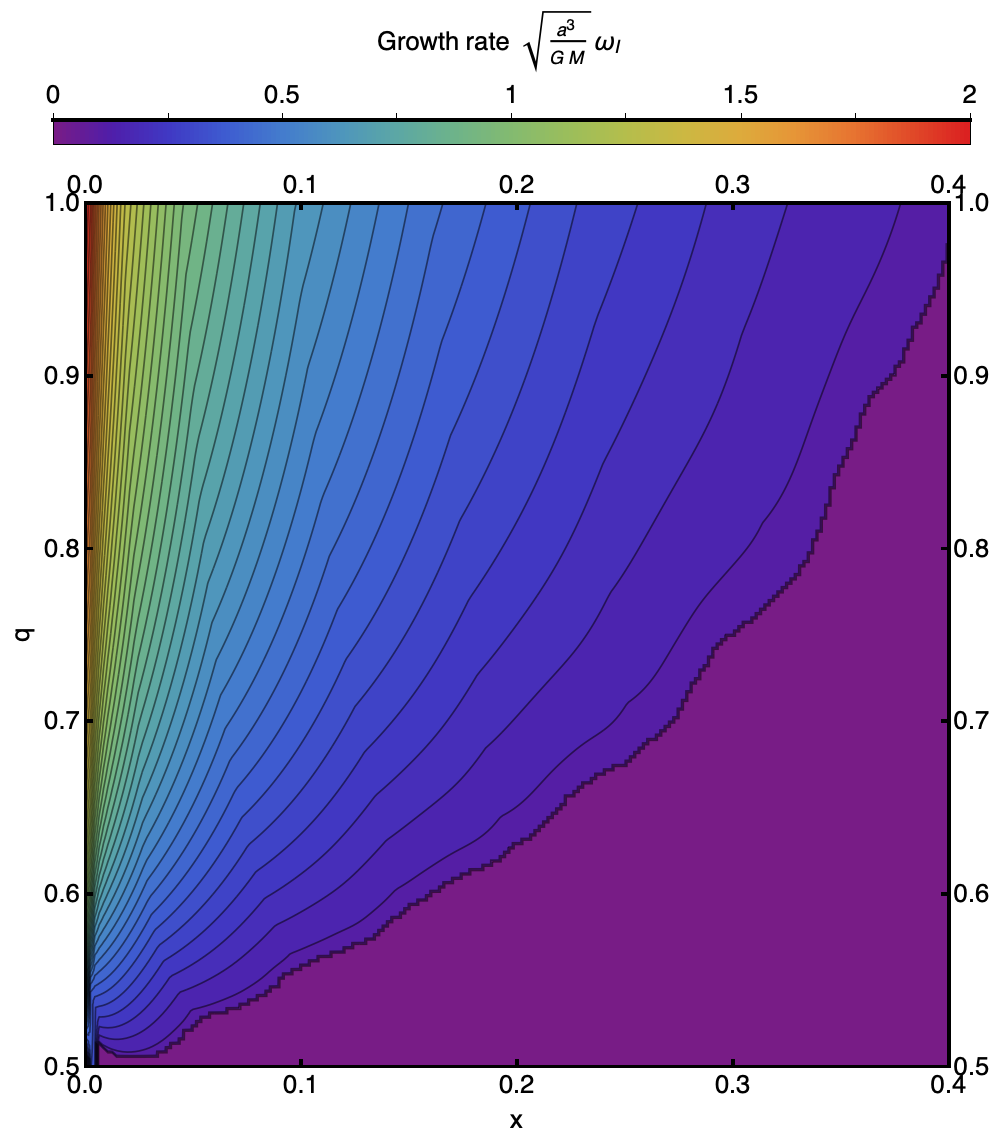
\includegraphics[width=0.6 \textwidth]{figs/growthRate_eps0_1.png}
   \caption{Growth rate (contour plot) at $\epsilon=0.1$ with $N=170$.}
   \label{fig:growthRate}
\end{figure}

\begin{figure}
    \centering
   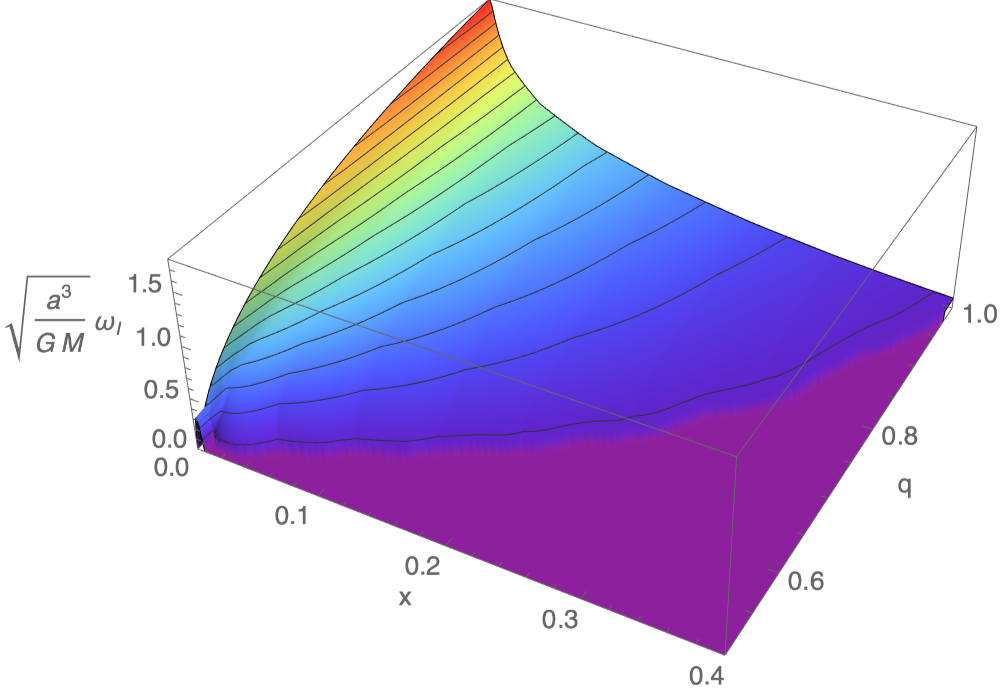
\includegraphics[width=0.6 \textwidth]{figs/growthRate3D_eps0_1.png}
   \caption{Growth rate (3D plot) at $\epsilon=0.1$ with $N=170$.}
   \label{fig:growthRate3D}
\end{figure}

Associated with the fastest growing eigenmode is an eigenvector, from which we can recover the over-density through
\begin{align}
(\Sigma)_m^p (r,\theta,t) &= \frac{M(1-x)}{2\pi a^2} \bigg(\frac{1-\xi}{2}\bigg)^{3/2} \sum_{n=|m|}^{\infty} \anm \hPnm(\xi) e^{i (m \theta- \omega t)} .
\end{align}

The corotation radius $r_{\mathrm{corot}}$ is defined by the equation $m \hOmega(r_{\mathrm{corot}}) = \Re(\homega)$.

\appendix

\section{General setting}

Consider a self gravitating disk with surface density $\Sigma$ and gravitational potential $\Phi$. Let $\bv$ be its velocity field and $P$ its pression field. Then it is described by the system
\begin{align}
&\frac{\partial \Sigma}{\partial t} + \bnab \cdot (\Sigma \bv) = 0 ,\\
&\frac{\partial \bv}{\partial t} + (\bv \cdot \bnab)(\bv) = -\frac{1}{\Sigma} \bnab P - \bnab \Phi ,\\
& \Delta \Phid = 4\pi G \Sigma \delta (z).
\end{align}
Here, $\Phi =\Phib^0+  \Phid +  \Phidh^0$. 
Suppose that we have a polytrope gas such that $P=\alpha \Sigma^{\Gamma}$ and let
\begin{equation}
\psi = \int \frac{\rd P(\Sigma)}{\Sigma} \Leftrightarrow \bnab \psi = \frac{\bnab P}{\Sigma}.
\end{equation}
 Then
 \begin{equation}
\psi = \frac{\alpha \Gamma}{\Gamma-1} \Sigma^{\Gamma-1}.
\end{equation}
 
 Letting $\Psi = \Phi + \psi$, we obtain
\begin{equation}
\frac{\partial \bv}{\partial t} + (\bv \cdot \bnab)(\bv) = - \bnab \Psi.
\end{equation}

%If $\Sigma_{\rm{disk}}\propto\Sigma_{\rm{DH}}$ then $q\in [1,+\infty[$ is constant and $q=1+\Mdh/\Md$. 
Let $x=\Mb/M$ and $q=\Md/(\Mdh+\Md) \in [0,1]$, where $M$ is the total stellar mass of the galactic disk+bulge.   Then

\begin{align*}
\Mb &= x M,\\
\Md &= (1 - x)M  ,\\
\Mdh &= \bigg(\frac{1}{q}-1\bigg) (1-x) M.
\end{align*}
%Therefore from the mass fractions we can obtain $x$ and $q$ by taking
%\begin{align*}
%x&=  \frac{\Md }{M},\\
%q &= 1+\frac{\Mdh/M}{\Md/M}  .
%\end{align*}
%with in particular $\Msg = \Md +\Mdh  = qx M$.
The system of equation can be rewritten as 
\begin{align}
&\frac{\partial \Sigma}{\partial t} + \frac{1}{r} \frac{\partial(r\Sigma \vr)}{\partial r} + \frac{1}{r} \frac{\partial(\Sigma \vt)}{\partial \theta} = 0 ,\\
&\frac{\partial \vr}{\partial t} + \vr \frac{\partial \vr}{\partial r} + \frac{\vt}{r} \frac{\partial \vr}{\partial \theta} - \frac{(\vt)^2}{r} = -\frac{\partial \Psi}{\partial r} ,\\
&\frac{\partial \vt}{\partial t} + \vr \frac{\partial \vt}{\partial r} + \frac{\vt}{r} \frac{\partial \vt}{\partial \theta} + \frac{\vr\vt}{r} = -\frac{1}{r}\frac{\partial \Psi}{\partial \theta} ,\\
& \Delta \Phid = 4\pi G \Sigma \delta (z).
\end{align}

 Let $\Phib^0 = - G \Mb/\sqrt{c^2+r^2}=- G  M x/\sqrt{c^2+r^2}$ with $x\in [0,1]$. An equilibrium state is given by the Plummer equilibrium, such that,  letting $\xi = (r^2-a^2)/(r^2+a^2) $, that is, $r/a=\sqrt{(1+\xi)/(1-\xi)}$,
\begin{align}
\vr^0 &= 0,\quad \quad (\vt^0)^2 = r \frac{\partial \Psi^0}{\partial r}, \\
%& \psi^0 = \frac{\kappa \Gamma}{\Gamma-1} (\Sigma^0)^{\Gamma-1} = \frac{\kappa \Gamma q^{\Gamma-1}}{(\Gamma-1)} (\Sigmad^0)^{\Gamma-1},\\
 \psi^0 &= \frac{\alpha \Gamma}{\Gamma-1} (\Sigma^0)^{\Gamma-1} ,\\
 \Sigma^0 &= \frac{\Md}{2\pi a^2} \frac{1}{(1+(r/a)^2)^{3/2}} =\frac{(1-x)M}{2\pi a^2}   \bigg(\frac{1-\xi}{2}\bigg)^{3/2},\\
 \Phidh^0 &= -\frac{G \Mdh}{a } \frac{1}{\sqrt{1+(r/a)^2}} = -\frac{G M(1-x)}{a }\bigg(\frac{1}{q}-1\bigg)   \bigg(\frac{1-\xi}{2}\bigg)^{1/2} ,\\
 \Phid^0 &= -\frac{G \Md}{a } \frac{1}{\sqrt{1+(r/a)^2}} = -\frac{G M (1-x)}{a } \bigg(\frac{1-\xi}{2}\bigg)^{1/2} ,\\
 \Phid^0+\Phidh^0 &= -\frac{G M (1-x)}{a q } \bigg(\frac{1-\xi}{2}\bigg)^{1/2} ,\\
\end{align}


Therefore, letting  $$\varepsilon_0 = \frac{U(x=0,q=1)}{|E(x=0,q=1)|} =\frac{3a \alpha \Gamma}{GM} \bigg(\frac{M}{2\pi a^2}\bigg)^{\Gamma-1},$$
and
$$\varepsilon = \frac{U_{\mathrm{disk}}}{|E_{\mathrm{disk}}|} =\frac{3a \alpha \Gamma}{G\Md} \bigg(\frac{\Md}{2\pi a^2}\bigg)^{\Gamma-1} = (1-x)^{\Gamma-2} \varepsilon_0,$$  we obtain 
\begin{align}
\Psi^0 &=  - \frac{G M x}{\sqrt{c^2+r^2}}-\frac{G M (1-x)}{a q}\bigg(\frac{1-\xi}{2}\bigg)^{1/2} + \frac{\alpha \Gamma}{(\Gamma-1)} (\Sigma^0)^{\Gamma-1} ,\\
{}&=  -\frac{G M x}{\sqrt{c^2+r^2}}+\frac{G M }{a} \bigg[-\frac{1-x}{q}\bigg(\frac{1-\xi}{2}\bigg)^{1/2} + \frac{\varepsilon_0 (1-x)^{\Gamma-1}}{3(\Gamma-1)}\bigg(\frac{1-\xi}{2}\bigg)^{3(\Gamma-1)/2} \bigg] ,\\
&=  \frac{G M(1-x)}{a}\bigg[-\frac{ ax}{c(1-x)}\frac{1}{ \sqrt{1+(r/c)^2}} - \frac{1}{q} \bigg(\frac{1-\xi}{2}\bigg)^{1/2} + \frac{\varepsilon_0  (1-x)^{\Gamma-2}}{3(\Gamma-1)}\bigg(\frac{1-\xi}{2}\bigg)^{3(\Gamma-1)/2} \bigg],\\
(\vt^0)^2 &= r \frac{\partial \Psi^0}{\partial r} =r \frac{\partial \Psi^0}{\partial \xi} \frac{\partial \xi}
{\partial r} = 4\bigg(\frac{r}{a}\bigg)^2    \bigg(\frac{1-\xi}{2}\bigg)^2 \frac{\partial \Psi^0}{\partial \xi}= (1+\xi) (1-\xi) \frac{\partial \Psi^0}{\partial \xi}  ,\\
&=\frac{GM(1-x)}{a}\bigg[\frac{ax}{c(1-x)}\bigg( \frac{r}{c}\bigg)^2 \bigg(\frac{1}{1+(r/c)^2}\bigg)^{3/2} 
+ \bigg(\frac{1+\xi}{2}\bigg) \bigg(\frac{1-\xi}{2}\bigg)^{1/2} \bigg(\frac{1}{q}-  \varepsilon_0 (1-x)^{\Gamma-2}\bigg(\frac{1-\xi}{2}\bigg)^{\frac{3\Gamma}{2}-2} \bigg)   \bigg], 
\end{align}
with
$$\frac{1-\xi}{2}= \frac{a^2}{r^2+a^2}= \frac{1}{1+(r/a)^2}; \quad \frac{1+\xi}{2}= \frac{r^2}{r^2+a^2}= \frac{(r/a)^2}{1+(r/a)^2}.$$

Note that for $x=0$ (only disk) and $q=1$ (purely self-gravitating system), we recover the expression of Toomre
\begin{align}
\vt^0 &=\bigg(\frac{GM}{a} \bigg)^{1/2}\bigg(\frac{1+\xi}{2}\bigg)^{1/2} \bigg(\frac{1-\xi}{2}\bigg)^{1/4}  \sqrt{1- \varepsilon \bigg(\frac{1-\xi}{2}\bigg)^{\frac{3\Gamma}{2}-2}} .
\end{align}

The perturbative equation at 1st order are
\begin{align}
&\frac{\partial \vr^p}{\partial t} + \frac{\vt^0}{r} \frac{\partial \vr^p}{\partial \theta} - 2\frac{\vt^0 \vt^p}{r} = -\frac{\partial \Psi^p}{\partial r} ,\\
&\frac{\partial \vt^p}{\partial t} + \vr^p \frac{\partial \vt^0}{\partial r} + \frac{\vt^0}{r} \frac{\partial \vt^p}{\partial \theta} + \frac{\vr^p\vt^0}{r} = -\frac{1}{r}\frac{\partial \Psi^p}{\partial \theta} ,\\
& \Delta \Phid^p = 4\pi G  \Sigma^p \delta (z), \\
& \psi^p =  \kappa \Gamma  (\Sigma^0)^{\Gamma-2} \Sigma^p .
\end{align}

We define $X^p(r,\theta,t) = \sum_{m\in \mathbb{Z}} X_m^p(r,t) e^{i m \theta}$ and look for a temporal dependency in $e^{-i \omega t}$.
Aoki \& Iye say that there is this following correspondance between surface density and gravitational potential through the Poisson equation:
\begin{align}
(\Sigma)_m^p (r,\theta) &= \frac{M(1-x)}{2\pi a^2} \bigg(\frac{1-\xi}{2}\bigg)^{3/2} \sum_{n=|m|}^{\infty} \anm \hPnm(\xi) e^{-i \omega t} ,\\
(\Phid)_m^p (r,\theta) &= -\frac{GM(1-x)}{a} \bigg(\frac{1-\xi}{2}\bigg)^{1/2} \sum_{n=|m|}^{\infty} \frac{\anm}{2n+1} \hPnm(\xi) e^{-i \omega t} ,\\
(\psi)_m^p (r,\theta) &= \alpha \Gamma \bigg(\frac{M}{2\pi a^2} \bigg)^{\Gamma-1} (1-x)^{\Gamma-1} \bigg(\frac{1-\xi}{2}\bigg)^{3/2(\Gamma-1)} \sum_{n=|m|}^{\infty} \anm \hPnm(\xi) e^{-i \omega t} ,\\
(\Psi)_m^p (r,\theta) &= \frac{GM(1-x)}{a } \bigg(\frac{1-\xi}{2}\bigg)^{1/2}\sum_{n=|m|}^{\infty} \bigg[\frac{\varepsilon_0(1-x)^{\Gamma-2} }{3} \bigg(\frac{1-\xi}{2}\bigg)^{\frac{3\Gamma}{2}-2}  -\frac{1}{2n+1}  \bigg]\anm \hPnm(\xi)e^{-i \omega t} .
\end{align}

Let us decompose the velocity components based on their equilibrium expression:
\begin{align}
(\vr)_m^p &= i \frac{m}{|m|} \bigg(\frac{GM(1-x)}{a}\bigg)^{1/2} \bigg(\frac{1+\xi}{2}\bigg)^{-1/2} \bigg(\frac{1-\xi}{2}\bigg)^{1/4} \sum_{n=|m|}^{\infty} \bnm \hPnm(\xi) e^{-i \omega t} ,\\
(\vt)_m^p &=\bigg(\frac{GM(1-x)}{a}\bigg)^{1/2} \bigg(\frac{1+\xi}{2}\bigg)^{-1/2} \bigg(\frac{1-\xi}{2}\bigg)^{1/4} \sum_{n=|m|}^{\infty} \cnm \hPnm(\xi) e^{-i \omega t} .
\end{align}

Letting $X_m^p = X^1  e^{-i \omega t}$, this yields the set of equations
\begin{align}
&i(-\omega + m \Omega)(\Sigmad)^1 + \frac{1}{r} \frac{\rd (r\Sigma_0 (\vr)^1)}{\rd r} + \frac{im\Sigma^0 (\vt)^1}{r} = 0,\\
&\frac{\rd (\Psi)^1}{\rd r} + i(-\omega + m \Omega)(\vr)^1 - 2 \Omega (\vt)^1 = 0,\\
&i m \frac{(\Psi)^1}{r} + \frac{\kappa^2}{2\Omega} (\vr)^1 + i(-\omega + m \Omega)(\vt)^1 = 0,
\end{align}
where $\Omega = \vt^0/r$ is the angular velocity and $\kappa^2=4\Omega^2[1+r/(2\Omega)\cdot(\rd \Omega /\rd r)]$ is the epicyclic frequency. Using the relation 
$$\int_{-1}^{1} \rd \xi \hPnm(\xi)\hPlm(\xi) = \delta_{nl},$$
and defining $\Omegaref=\sqrt{GM/a^3 }$, $\Sigmaref=M/(2\pi a^2)$   such that $\homega = \omega/\Omegaref$, $\hOmega = \Omega/\Omegaref$, $\hkappa = \kappa/\Omegaref$, $\hSigma=\Sigma/\Sigmaref$ and $\lambda=\frac{|m|}{m}\homega$, we obtain the matrix equations
\begin{align}
&\sum_{n=|m|}^{\infty}  A_{ln} \anm  +\sum_{n=|m|}^{\infty}  B_{ln}\bnm+\sum_{n=|m|}^{\infty}  C_{ln}\cnm= \lambda \alm ,\\
&\sum_{n=|m|}^{\infty}D_{ln}\anm + \sum_{n=|m|}^{\infty}   A_{ln} \bnm+  \sum_{n=|m|}^{\infty} F_{ln} \cnm  =  \lambda    \blm ,\\
&\sum_{n=|m|}^{\infty}G_{ln}\anm + \sum_{n=|m|}^{\infty}   H_{ln} \bnm+  \sum_{n=|m|}^{\infty} A_{ln} \cnm  =  \lambda    \blm ,
 \end{align}
where we defined
\begin{align}
A_{ln} &= |m| \int_{-1}^{1} \rd \xi  \hPlm(\xi)\hOmega(\xi)\hPnm(\xi) , \\
B_{ln} &= 4 {\sqrt{1-x}} \int_{-1}^{1} \rd \xi  \hPlm(\xi) \bigg(\frac{1-\xi}{2}\bigg)^{1/2} \frac{\rd}{\rd \xi} \bigg[\bigg(\frac{1-\xi}{2}\bigg)^{5/4}\hPnm(\xi)\bigg], \\
C_{ln} &= |m| {\sqrt{1-x}} \int_{-1}^{1} \rd \xi \hPlm(\xi) \bigg(\frac{1-\xi}{2}\bigg)^{3/4}\bigg(\frac{1+\xi}{2}\bigg)^{-1}   \hPnm(\xi), \\
D_{ln} &= 4 {\sqrt{1-x}} \int_{-1}^{1} \rd \xi \hPlm(\xi)  \bigg(\frac{1-\xi}{2}\bigg)^{5/4} \bigg(\frac{1+\xi}{2}\bigg) \\
&\times\frac{\rd}{\rd \xi} \bigg[\bigg(\frac{1}{2n+1}-\frac{\varepsilon_0(1-x)^{\Gamma-2} }{3} \bigg(\frac{1-\xi}{2}\bigg)^{\frac{3\Gamma}{2}-2} \bigg) \bigg(\frac{1-\xi}{2}\bigg)^{1/2}\hPnm(\xi) \bigg] ,\\
F_{ln} &=2  \int_{-1}^{1} \rd \xi  \hPlm(\xi)\hOmega(\xi)\hPnm(\xi) , \\
G_{ln} &= -|m|{\sqrt{1-x}} \int_{-1}^{1} \rd \xi \hPlm(\xi)  \bigg(\frac{1-\xi}{2}\bigg)^{3/4} 
\bigg(\frac{1}{2n+1}-\frac{\varepsilon_0(1-x)^{\Gamma-2} }{3} \bigg(\frac{1-\xi}{2}\bigg)^{\frac{3\Gamma}{2}-2} \bigg) \hPnm(\xi)  ,\\
H_{ln} &= \int_{-1}^{1} \rd \xi  \hPlm(\xi)\frac{\hkappa^2(\xi)}{2\hOmega(\xi)}\hPnm(\xi) .
\end{align}
with
\begin{align}
\hOmega(\xi) &=\sqrt{\frac{1-\xi}{1+\xi}} \sqrt{\frac{a}{c}\frac{x}{(1-x)}\bigg( \frac{r}{c}\bigg)^2 \bigg(\frac{1}{1+(r/c)^2}\bigg)^{3/2} 
+ \bigg(\frac{1+\xi}{2}\bigg) \bigg(\frac{1-\xi}{2}\bigg)^{1/2}  \bigg[\frac{1}{q}-  \varepsilon_0 (1-x)^{\Gamma-2}\bigg(\frac{1-\xi}{2}\bigg)^{\frac{3\Gamma}{2}-2} \bigg] } ,\\
\frac{\hkappa^2(\xi)}{2\hOmega(\xi)} &= 2\hOmega(\xi) \bigg[1+\frac{r}{2\hOmega}\frac{\rd \hOmega }{\rd r}\bigg] = 2\hOmega(\xi) \bigg[1+\frac{(1+\xi)(1-\xi)}{2\hOmega}\frac{\rd \hOmega }{\rd \xi} \bigg],
\end{align}
where
$$\frac{\rd(r/a)}{\rd \xi} = \frac{\rd}{\rd \xi} \bigg[\sqrt{\frac{1+\xi}{1-\xi}}\bigg] = (1-\xi)^{-3/2}(1+\xi)^{-1/2}$$

Since $(r/c)^2 = (a/c)^2 \cdot (r/a)^2 =  (a/c)^2 \cdot (1+\xi)/(1-\xi)$, we have that
\begin{align}
\hOmega(\xi) &=\bigg(\frac{1-\xi}{2}\bigg)^{3/4}  \sqrt{\bigg( \frac{a}{c}\bigg)^3\frac{x}{1-x} \bigg(\frac{1-\xi}{2}\bigg)^{-3/2} \bigg(\frac{1}{1+(r/c)^2}\bigg)^{3/2} 
+   \bigg(\frac{1}{q}-  \varepsilon_0 (1-x)^{\Gamma-2}\bigg(\frac{1-\xi}{2}\bigg)^{\frac{3\Gamma}{2}-2} \bigg) } .
\end{align}



\end{document}
